\section{MTB-2-AVR}

Aby nebylo nutné všechny současné \gls{mtbuni} desky vyměňovat za desky nové,
je třeba staré desky povýšit tak, aby podporovaly nový protokol \gls{mtbuni} v4.
Díky omezenosti procesoru v současných modulech \gls{mtbuni} není možné tuto
úpravu provést pouze změnou firmwaru, viz \ref{prev}.

Výhodou je, že procesory na současných \gls{mtbuni} modulech jsou v
\textit{DIL} patici. Nabízí se tedy přirozená cesta najít nový procesor
odpovídajícího rozložení pinů. Procesor, který by měl vyhovující rozložení pinů
a požadované parametry bohužel neexistuje. Uvažován byl například procesor
TODO. Proto se autor této práce vydal cestou výroby nástavné desky, která se
zasune do \textit{DIL} patice současné \gls{mtbuni} desky a na sobě bude mít
\textit{smd} procesor.  Správné napojení pinů se vyřeší na nástavné desce
plošných spojů.

Tuto myšlenku implementuje deska \textit{MTB-2-AVR}, viz obrázek
\ref{fig:mtb-2-avr-alone}.

\begin{figure}[ht]
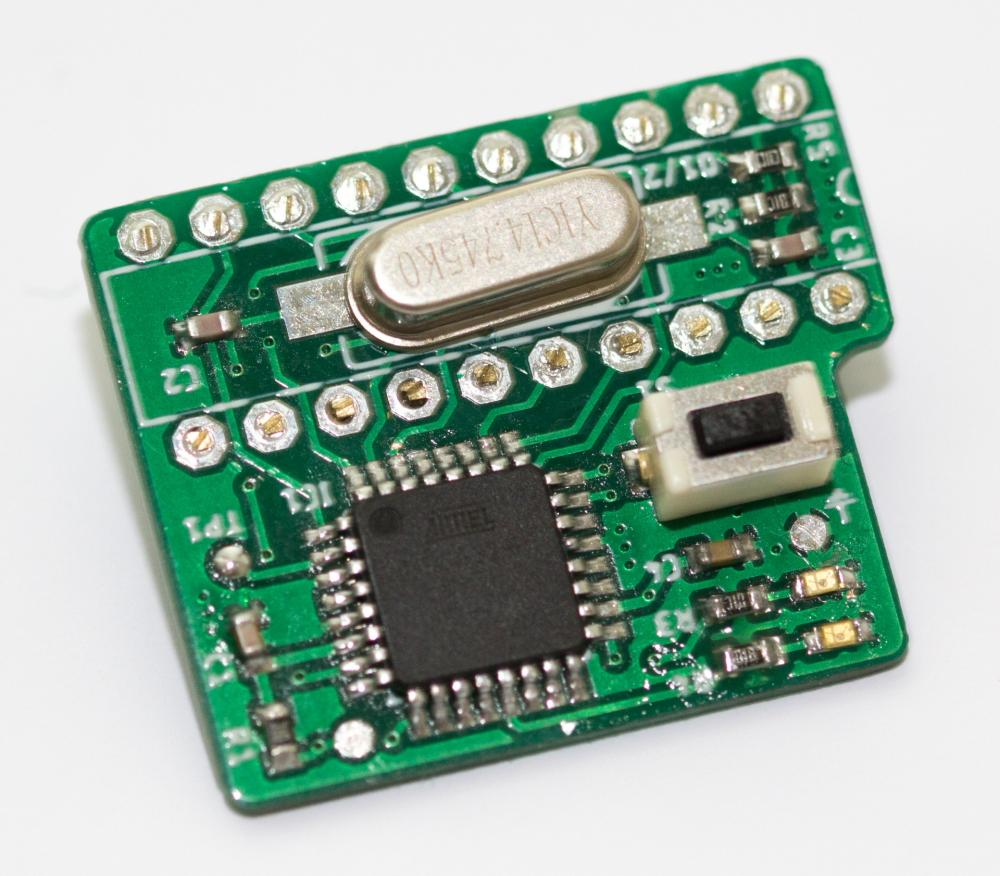
\includegraphics[width=0.4\textwidth]{data/uni-2-upgrade-alone.jpg}
\caption{Nástavná deska \textit{MTB-2-AVR}.}
\label{fig:mtb-2-avr-alone}
\end{figure}

\begin{figure}[ht]
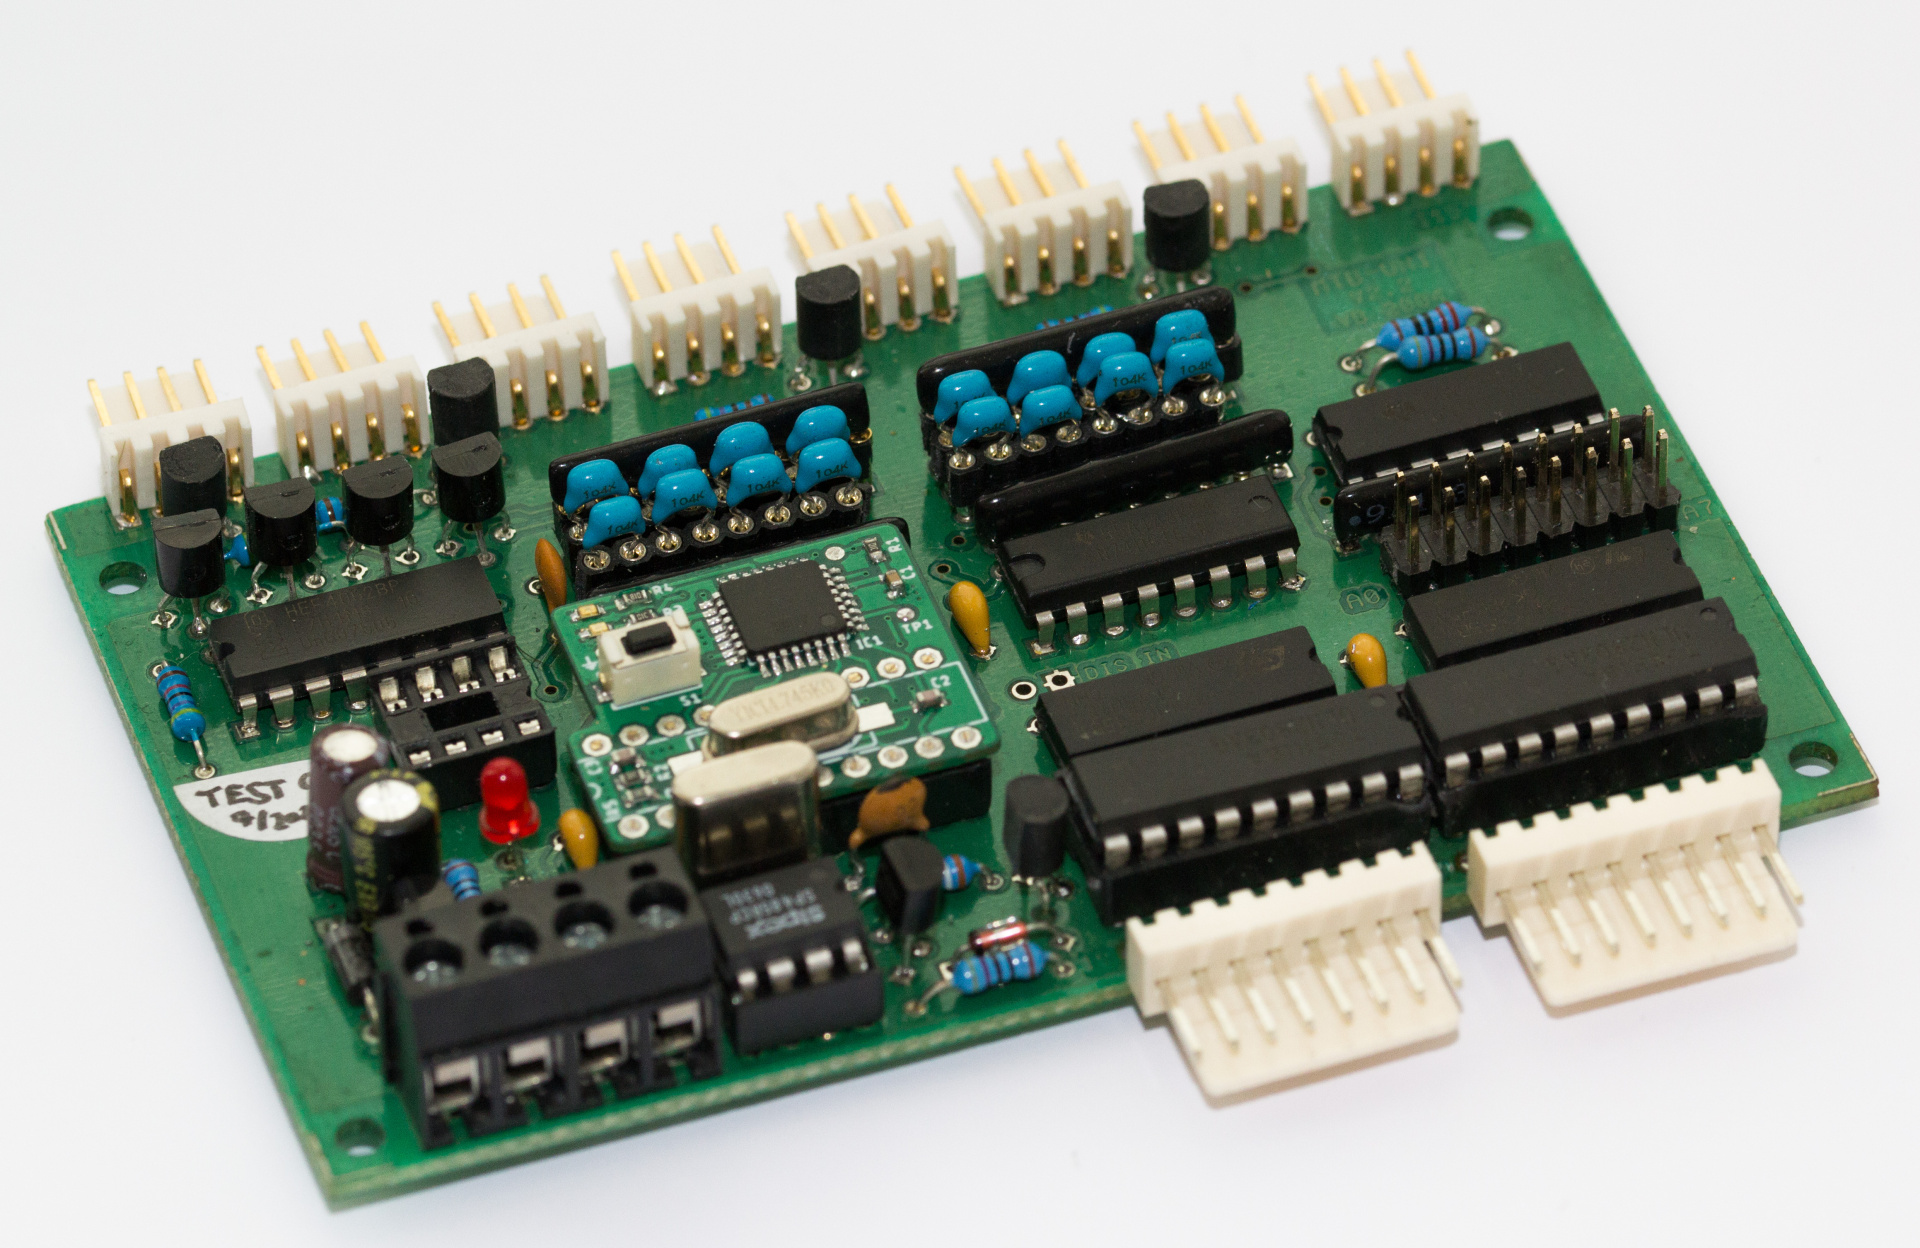
\includegraphics[width=0.9\textwidth]{data/uni-2-upgrade-all.jpg}
\caption{Nástavná deska \textit{MTB-2-AVR} v modulu \gls{mtbuni} v2.}
\label{fig:mtb-2-avr-inside}
\end{figure}

Deska je navržena tak, aby se dala umístit místo procesoru libovolného z modulů
\gls{mtbuni}, \textit{MTB-UNIm} a \textit{MTB-TTL}. Srdcem desky je procesor
\textit{ATmega328p} autorovy oblíbené architektury procesorů \textit{AVR}.
Konkrétně tento model byl zvolen, protože obsahuje dostatečnou kapacitu paměti
na bootloader a protože jej \textit{Jlcpcb} má mezi \textit{basic součástkami}
(viz \ref{todo}).

Schéma a deska plošných spojů jsou vyvinuty jako openhardware projekt a dostupné
na \url{https://github.com/kmzbrnoI/mtb-2-avr-pcb}. Deska plošných spojů obsahuje
kromě procesoru chybějící LED, aby každá \gls{mtb} deska měla zelenou, žlutou a
červenou LED. Dále obsahuje krystal, protože původní krystal na \gls{mtbuni}
desce je mimo rozsah dovolených hodnot kmitočtů krystalu pro procesor
\textit{ATmega328p}. Deska dále obsahuje tlačítko (pro unifikaci hardwaru
s~\gls{mtbuni} v4 modulem).

Jak již bylo zmíněno, tato nástavá deska se bude osazovat do patic současných
\gls{mtbuni} i \textit{MTB-TTL} desek. Přitom u \gls{mtbuni} desek by měl procesor
podporovat IR čidla na vstupech. Procesor proto detekuje v jaké desce se nachází
(byl identifikován a využit HW rozdíl různých typů desek) a podle toho buď
zapne nebo vypne podporu IR čidel. Do počítače pak přes \gls{mtbbus} protokol
nahlásí, jestli IR čidla podporuje nebo ne.

Zde mimochodem využijeme \textit{Module specific command} (\ref{}). Modulu
\textit{MTB-2-AVR} lze poslat příkaz, aby znovu provedl autodetekci typu
desky, do které je vložené, případně nastavit typ desky ručně.

Firmware je pod opensource licencí dostupný na
\url{https://github.com/kmzbrnoI/mtb-2-avr-fw}. Firmware se opět skládá
z bootloaderu a hlavního programu.
